%--------------------
% Packages
% -------------------
\documentclass[10pt,a4paper]{article}
% \usepackage[a4paper, left=15mm, right=15mm, top=15mm, bottom=15mm]{geometry}
\usepackage[utf8x]{inputenc}
\usepackage[T1]{fontenc}
%\usepackage{gentium}
\usepackage{mathptmx} % Use Times Font
% \usepackage[siunitx]{circuitikz} % for circuit schematics
\usepackage{siunitx}
\usepackage{amsmath} % for the equation* environment


\usepackage[pdftex]{graphicx} % Required for including pictures % clashes with circuitikz
% \usepackage[swedish]{babel} % Swedish translations
\usepackage[pdftex,linkcolor=black,pdfborder={0 0 0}]{hyperref} % Format links for pdf
\usepackage{calc} % To reset the counter in the document after title page
\usepackage{enumitem} % Includes lists

\frenchspacing % No double spacing between sentences
\linespread{1.2} % Set linespace
\usepackage[a4paper, lmargin=0.1\paperwidth, rmargin=0.1\paperwidth, tmargin=0.1\paperheight, bmargin=0.1\paperheight]{geometry} %margins
%\usepackage{parskip}
% \usepackage[all]{nowidow} % Tries to remove widows
\usepackage[protrusion=true,expansion=true]{microtype} % Improves typography, load after fontpackage is selected

\usepackage[inkscapelatex=false]{svg}
\graphicspath{ {./media/} }


%-----------------------
% Set pdf information and add title, fill in the fields
%-----------------------
\hypersetup{ 	
pdfsubject = {},
pdftitle = {ee5311-2025-ee24s053-pwc-report-tut2},
pdfauthor = {Karthik B K <ee24s053@smail.iitm.ac.in>}
}

%-----------------------
% Begin document
%-----------------------
\begin{document}

\title{EE5311 \\ Report of Practical Work Conducted for Tutorial 02}
\author{Karthik B K ee24s053}
\maketitle

\section{Experiment 01}
\subsection{Calculations}
In the given circuit schematic, we know from visual inspection that the pMOS's region of operation will be \emph{saturation} and that of the nMOS will be \emph{linear}. With that information, we equate the currents in the said regions of operations as follows:

\begin{center}
    $I_{d,sat,p} = I_{d,lin,n}$ \\
    $\frac{1}{2}\mu_{p}C_{ox}(\frac{W}{L})_{p}\frac{E_{C}(V_{gs}-V_{tp})^{2}}{V_{gs}-V_{tp}+E_{C}}(1+\lambda_{p} V_{ds}) = \frac{1}{2}\mu_{n}C_{ox}(\frac{W}{L})_{n}\frac{1}{1+(\frac{V_{ds}}{E_{C}})}(2(V_{gs}-V_{tn})V_{ds}-V_{ds}^2)(1+\lambda_{n} V_{ds})$
\end{center}

\noindent We use the values provided in the problem statement, and obtain:

\begin{center}
    $(\frac{W}{L})_{p} = 1.610$
\end{center}

\noindent Since the minimum width of a 3-terminal pMOS transistor in the given sky130 standard cell library is $0.42 \mu m$, we want to increase the length of our pMOS device to meet this aspect ratio. Hence, we would size the pMOS transistor as follows:

\begin{center}
    $W_{p} = 0.42 \mu m, L_{p} = 0.26 \mu m$
\end{center}

\noindent In order to compute the noise margins, we first compute $V_{IH}$ and $V_{IL}$ as follows:

\begin{center}
    $V_{IL} = V_{tn} + \frac{1}{R_L(2k_n\frac{W_n}{L_n})}$ \\
    $V_{IH} = V_{tn} + \sqrt{\frac{4V_{DD}}{3K_nR_L\frac{W_n}{L_n}}} - \frac{1}{2K_nR_L\frac{W_n}{L_n}}$
\end{center}

\noindent We use the values provided in the problem statement, and obtain:

\begin{center}
    $V_{IL} = 0.765 mV$ \\
    $V_{IH} = 1196 mV$ \\

    thus, $NM_L = 0.765 V$ and $NM_H = 0.604 V$
\end{center}

\noindent In order to compute average power at a constant onput voltage level, $V+{in} = V_{DD}$, we can simply measure the current drawn from the voltage source $V_{DD}$ and multiply it with the maginitude of the supply voltage level, $1.8V$. In order to do so, we measure the drain currents through both MOS devices and apply KCL at the output node:

\begin{center}
    $I_{d,sat,p} = \frac{1}{2}\mu_{p}C_{ox}(\frac{W}{L})_{p}\frac{E_{C}(V_{gs}-V_{tp})^{2}}{V_{gs}-V_{tp}+E_{C}}(1+\lambda_{p} V_{ds})$ and \\
    $I_{d,lin,n} = \frac{1}{2}\mu_{n}C_{ox}(\frac{W}{L})_{n}\frac{1}{1+(\frac{V_{ds}}{E_{C}})}(2(V_{gs}-V_{tn})V_{ds}-V_{ds}^2)(1+\lambda_{n} V_{ds})$
\end{center}

\noindent We use the values provided in the problem statement, and obtain:

\begin{center}
    $I_{d,sat,p} = -86.1 \mu A$ and \\
    $I_{d,lin,n} = 291.9 \mu A$ \\
    thus, $I_{out} = -291.1 \mu A$ \\
    indicating $P_* = abs(I_{out}) * V_{DD} = 678.8 \mu W$
\end{center}

\noindent Since the output voltage level is expected to be low, a negative direction of the current at the output node would indicate that the load is discharging.

\subsection{Schematics}
\noindent We draw the following schematic using \emph{xschem}.
\newline
\begin{center}
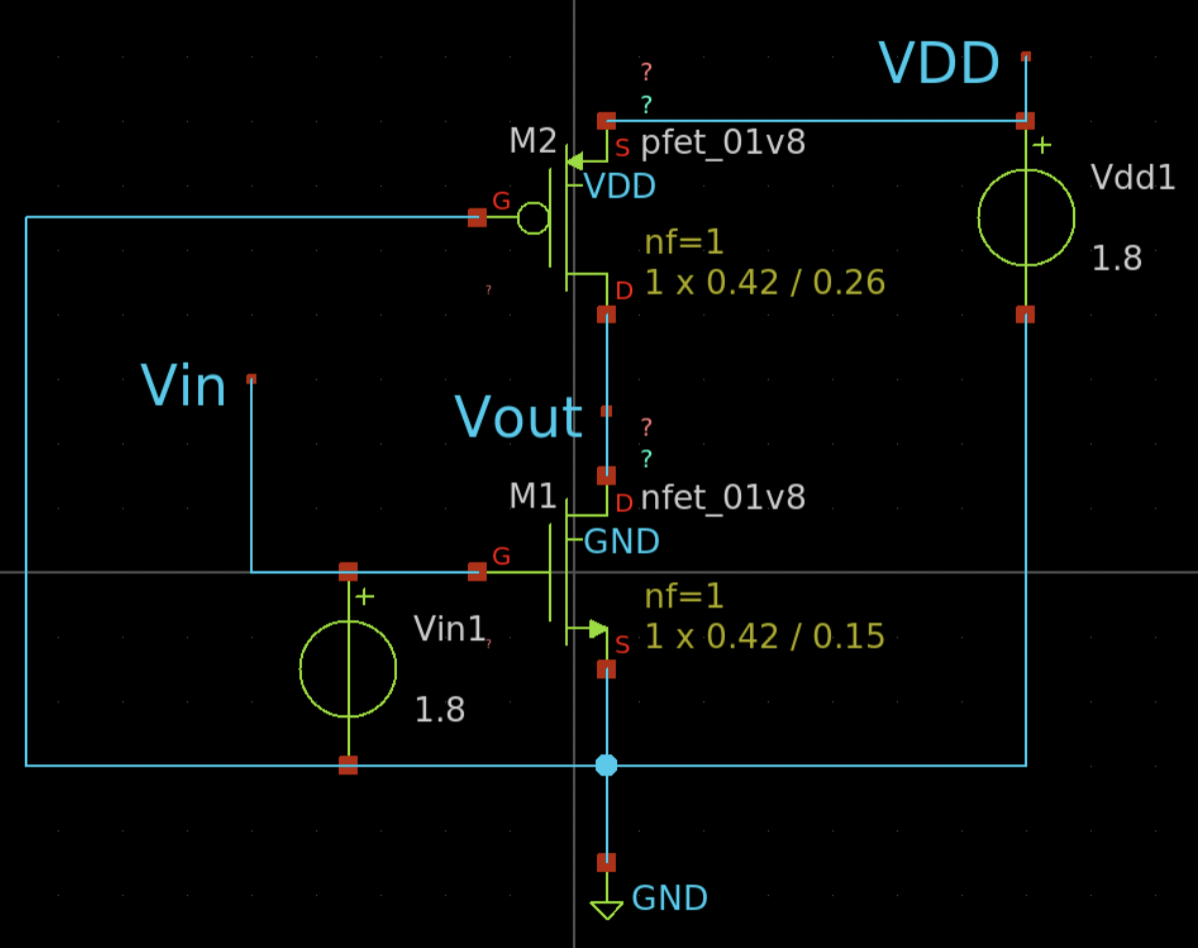
\includegraphics[scale=0.4]{tut2/reports/media/expt1.sch.png}
\end{center}


\subsection{Measurements}

\noindent We plot the voltage transfer charecteristics for the said inverter using a SPICE simulation and obtain the following plot:

\begin{center}
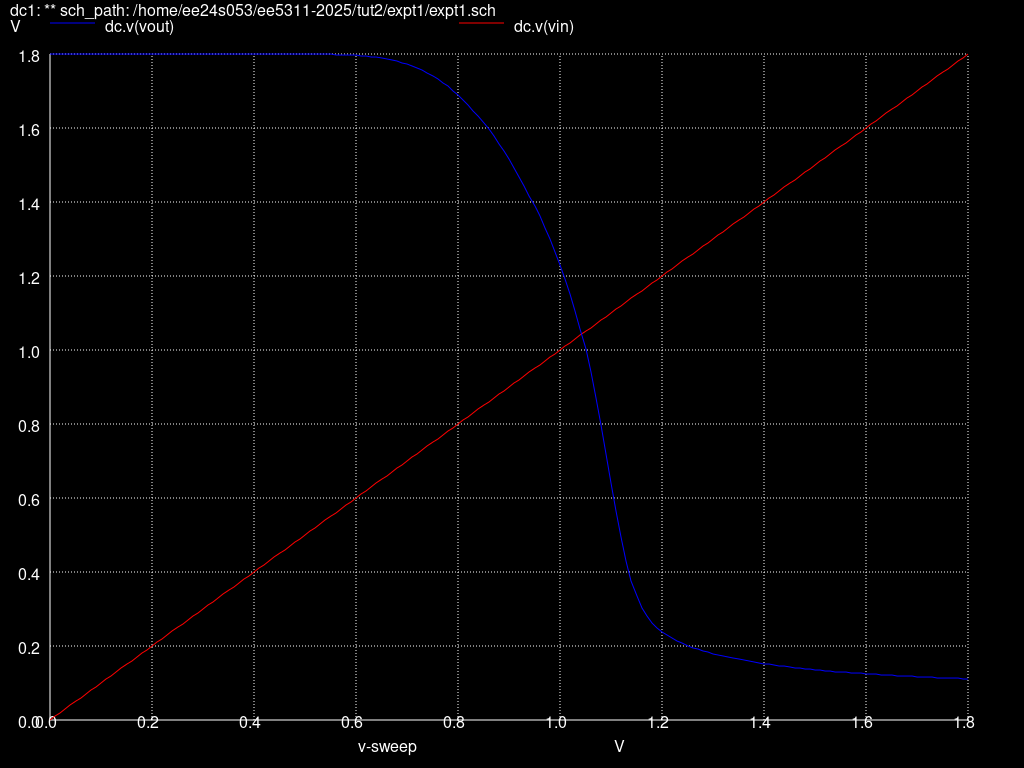
\includegraphics[scale=0.3]{tut2/reports/media/expt1_vtc.png}
\end{center}

\noindent We measure the inverter threshold voltage, defined as the magnitude of input voltage for which the output voltage is half of the supply voltage, as follows:

\begin{verbatim}
    meas dc Vtinv when v(Vout)=0.9 cross=1
\end{verbatim}

\noindent We observe that the inverter voltage is: $1.06587$ V.\newline
We also plot the first-order derivative of the output voltage curve using a SPICE simulation and obtain the following plot:

\begin{center}
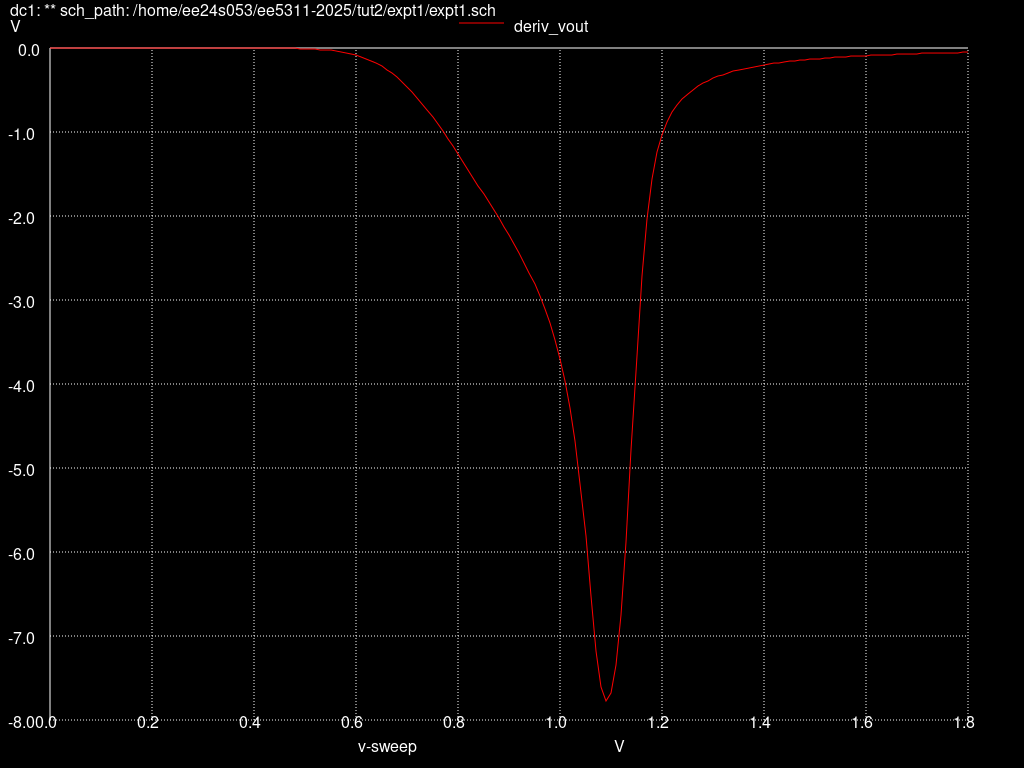
\includegraphics[scale=0.3]{tut2/reports/media/expt1_deriv_vout.png}
\end{center}

\noindent We measure the input voltage levels, $Vil, Vih$, as follows:

\begin{verbatim}
    let deriv_vout = deriv(v(Vout))
    meas dc Vil when deriv_vout=-1 cross=1
    meas dc Vih when deriv_vout=-1 cross=2
\end{verbatim}

\noindent We obtain the following values:

\begin{verbatim}
    vil = 7.707750e-01
    vih = 1.202181e+00
\end{verbatim}

\noindent Using these values for $Vil, Vih$, we compute the noise margins, $NM_{L}$ and $NM_{H}$ to be:

\begin{verbatim}
    NML: 0.770775
    NMH: 0.597819
\end{verbatim}

\noindent Given that $V_{in} = V_{dd}$, we can say that the average power consumed will be equal to the peak power consumed, which is $P_* = I_{out} * V_{dd}$. In order to compute this, we \emph{simply} fix the input voltage level to what is asked, $V_{dd}$ and measure the current drawn from the supply voltage. We plot the output current throughout the DC sweep, and measure the value of current at the said input voltage level. We obtain the following plot:

\begin{center}
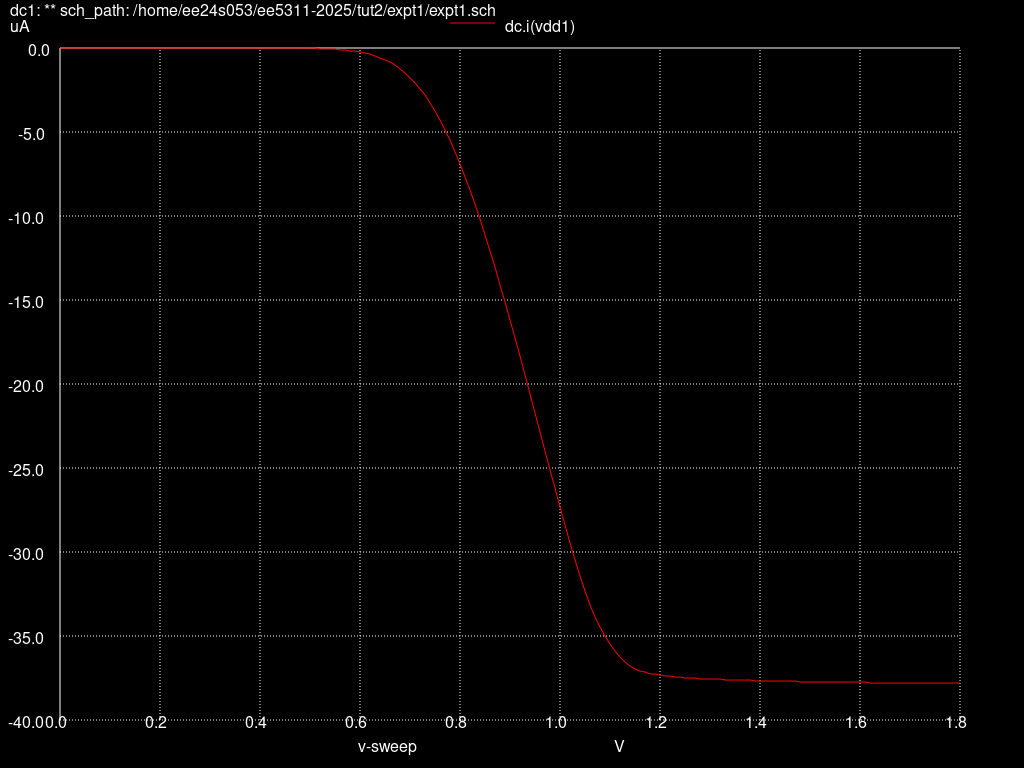
\includegraphics[scale=0.3]{tut2/reports/media/expt1_iout.png}
\end{center}

\noindent At $V_{in} = V_{dd}$, we obtain the following measurement for the current:

\begin{verbatim}
    Iout = 3.781284e-05
\end{verbatim}

\noindent Hence,
\begin{center}
    $P_* = 3.781 * 10^{-5} * 1.8 W = 6.805 * 10^{-5} W$
\end{center}
The average power consumed when $V_{in} = V_{dd}$ is:
\begin{center}
    $P_* = 68.05 \mu W$
\end{center}

\section{Experiment 02}
\subsection{Calculations}
\noindent When the inverter threshold voltage level is made to be half that of the supply voltage, $V_{tinv} = V_{m} = \frac{V_{DD}}{2}$, the pull-up transistor would have $abs(V_{gs,p}) = \frac{V_{dd}}{2} = 0.9V$. This will drive both the transistors into an active state. That is, both transistors will be turned on. The pull-up transistor will operate in the \emph{saturation} since $V_{DS,p} > V_{d,sat,p}$. The pull-down transistor will operate in the \emph{linear} region, since $V_{DS,n} \leq V_{d,sat,n}$. We equate the expressions for drain current for both transistors in the aforementioned regions of operation:

\begin{center}
    $I_{d,sat,p} = I_{d,lin,n}$ \\
    $\frac{1}{2}\mu_{p}C_{ox}(\frac{W}{L})_{p}\frac{E_{C}(V_{gs}-V_{tp})^{2}}{V_{gs}-V_{tp}+E_{C}}(1+\lambda_{p} V_{ds}) = \frac{1}{2}\mu_{n}C_{ox}(\frac{W}{L})_{n}\frac{1}{1+(\frac{V_{ds}}{E_{C}})}(2(V_{gs}-V_{tn})V_{ds}-V_{ds}^2)(1+\lambda_{n} V_{ds})$
\end{center}

\noindent We use the values provided in the problem statement, and obtain:

\begin{center}
    $(\frac{W}{L})_{p} = 1.610$
\end{center}

\noindent In order to retain symmetricity in sizing, we will size the pMOS to be twice as large as the nMOS device. Hence, $W_p = 0.84 \mu m$ and $L_p = 0.15 \mu m$. The nMOS device remains to be a minimum-sized transistor.

\subsection{Schematics}
\noindent We draw the following schematic using \emph{xschem}:
\begin{center}
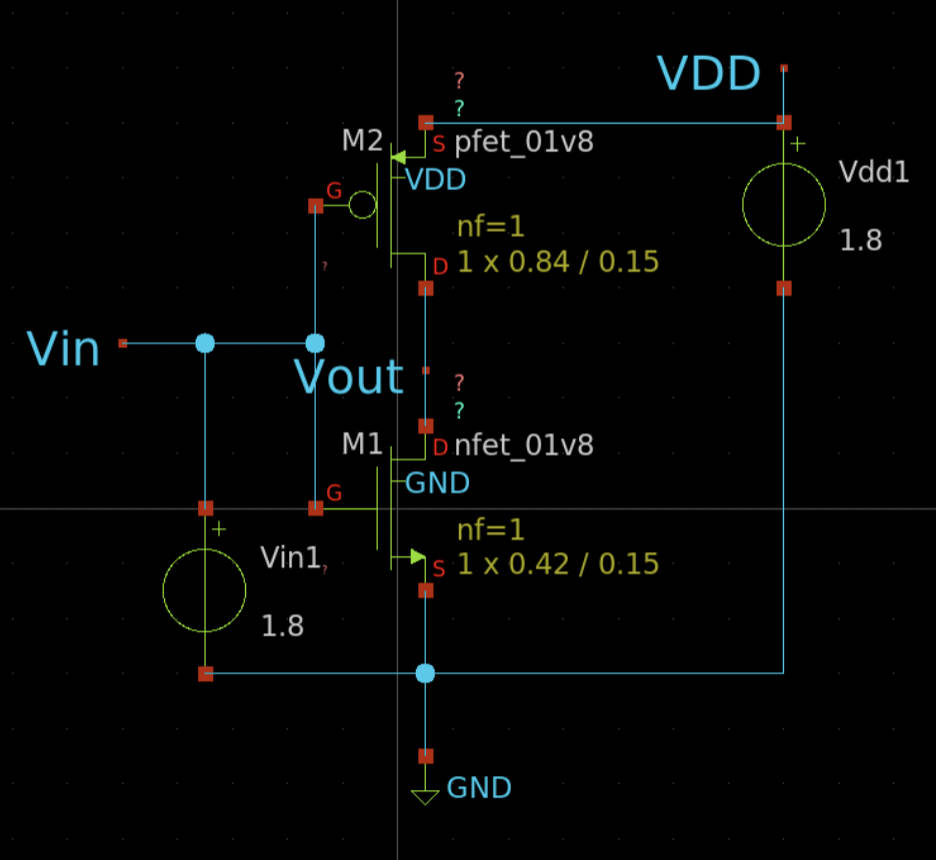
\includegraphics[scale=0.5]{tut2/reports/media/expt2_0.sch.png}
\end{center}

\subsection{Measurements}
\noindent We obtain the following plot for voltage transfer charecteristics:
\begin{center}
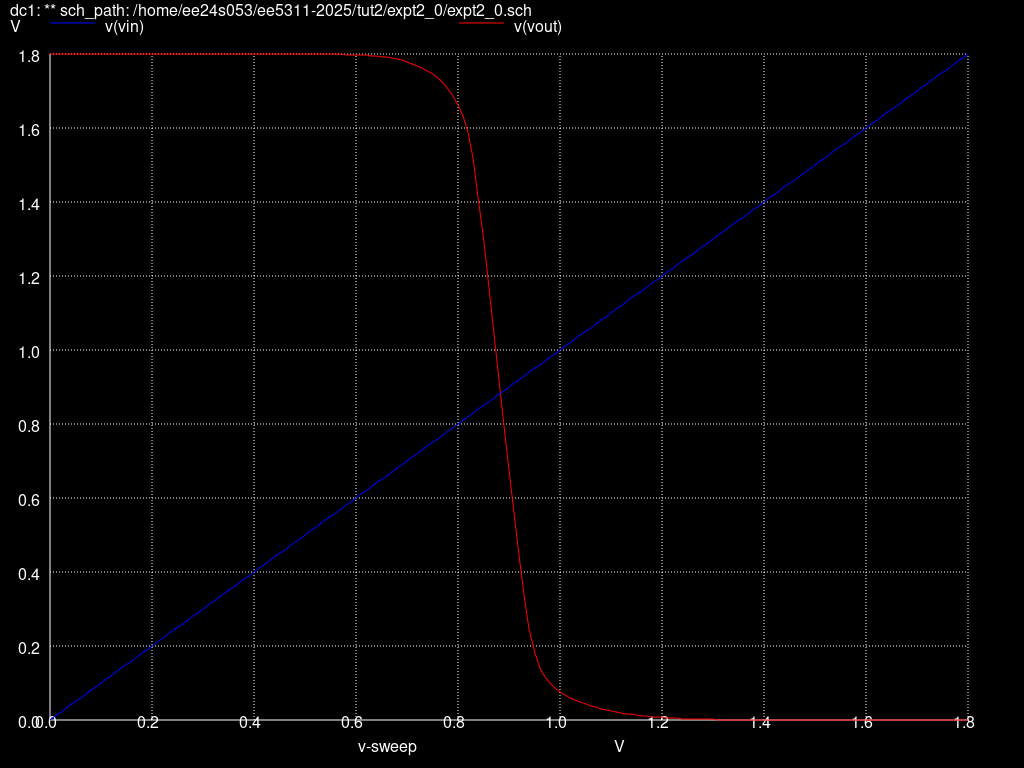
\includegraphics[scale=0.3]{tut2/reports/media/expt2_0_vtc.png}
\end{center}

\noindent We obtain the following plot for the derivative of the output voltage level:
\begin{center}
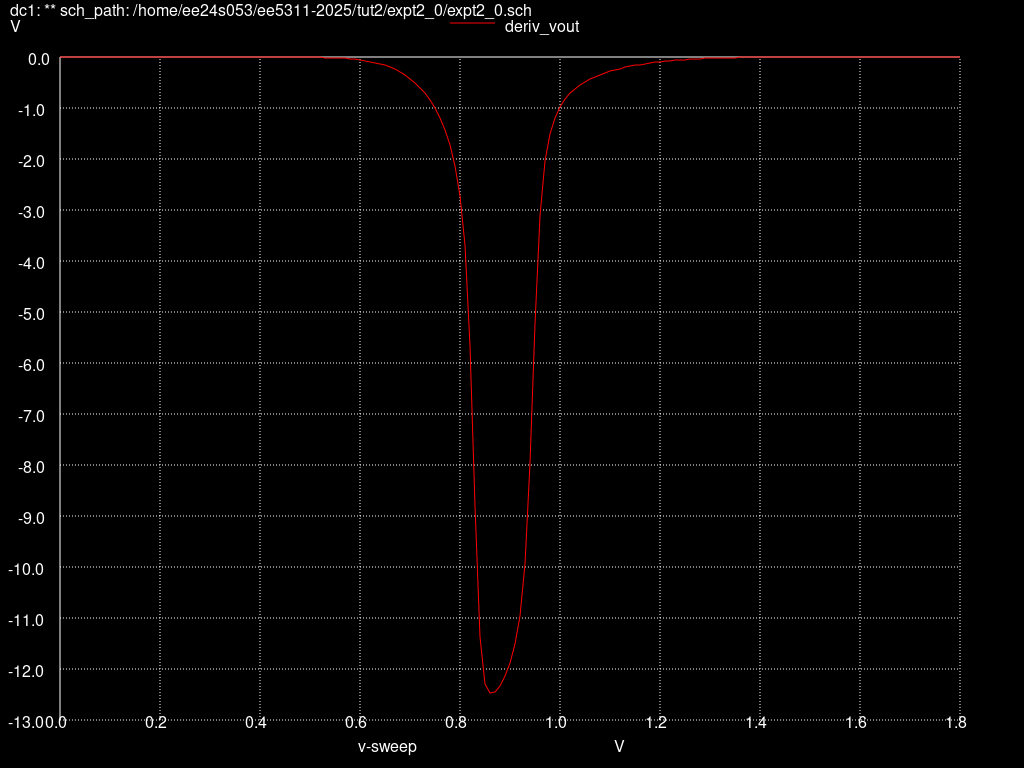
\includegraphics[scale=0.3]{tut2/reports/media/expt2_0_deriv_vout.png}
\end{center}

\noindent We make the following measurements from the plotted curve:

\begin{center}
    $V_{IL} = 750.0234 mV$ \\
    $V_{IH} = 999.1007 mV$ \\
    $V_m = 881.4951 mV$ \\
    thus, $NM_L = 750.023 mV$ and $NM_H = 800.899 mV$
\end{center}

\noindent We modify the simulation setup to sweep the supply voltage level from $0.2V$ to $1.8V$ in steps of $0.2V$. We obtain the following voltage transfer charecteristics:
\begin{center}
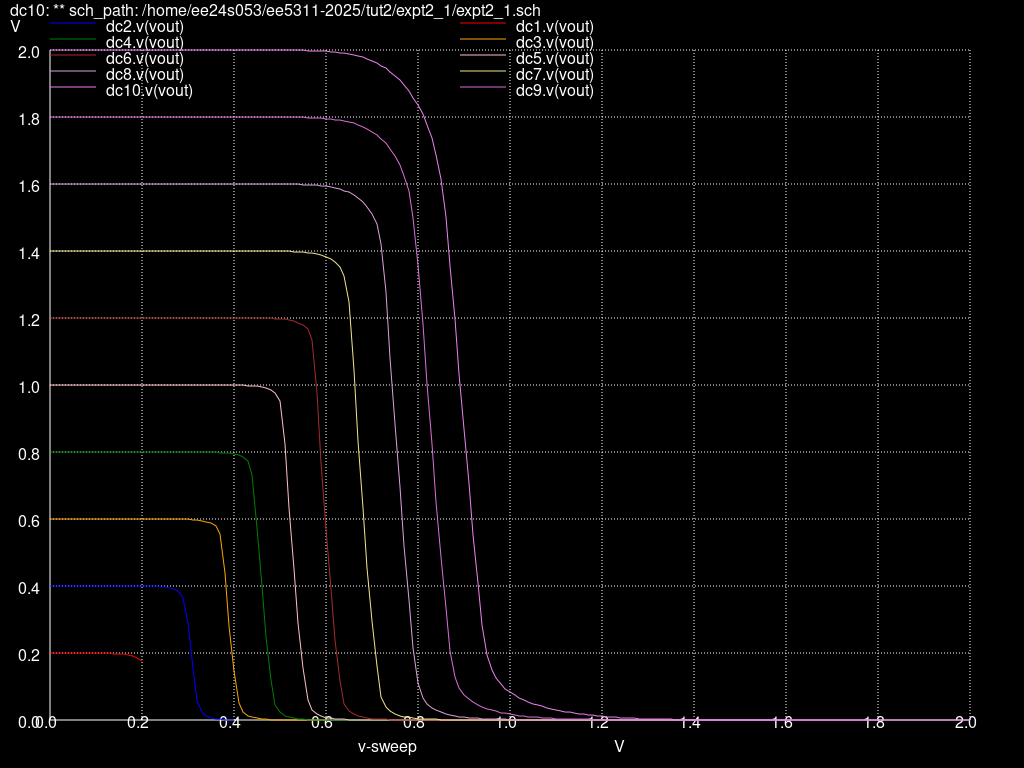
\includegraphics[scale=0.3]{tut2/reports/media/expt2_1_vtc.png}
\end{center}

\noindent We now analyze the current that charges the output at three distinct voltage levels; $0.2V$ (sub-threshold), $0.8V$ (near-threshold), and $1.8V$ (super-threshold):
\begin{center}
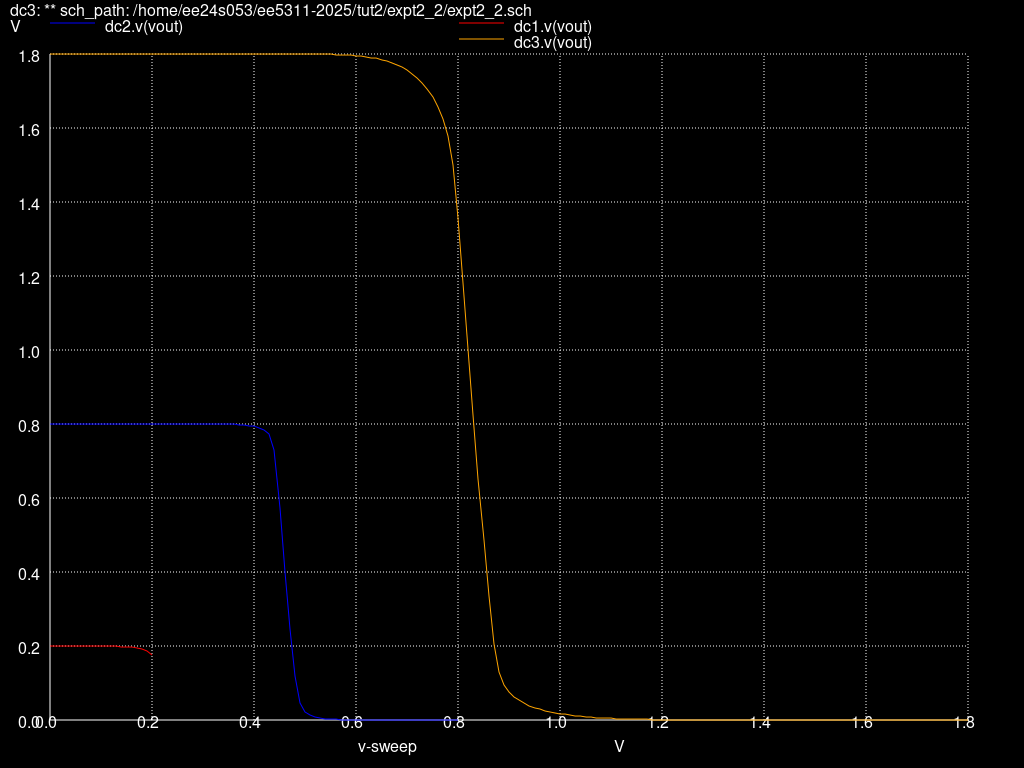
\includegraphics[scale=0.3]{tut2/reports/media/expt2_2_vtc.png}
\end{center}

\noindent We obtain the following plots for drain currents when operating at the said three voltage levels:

\begin{center}
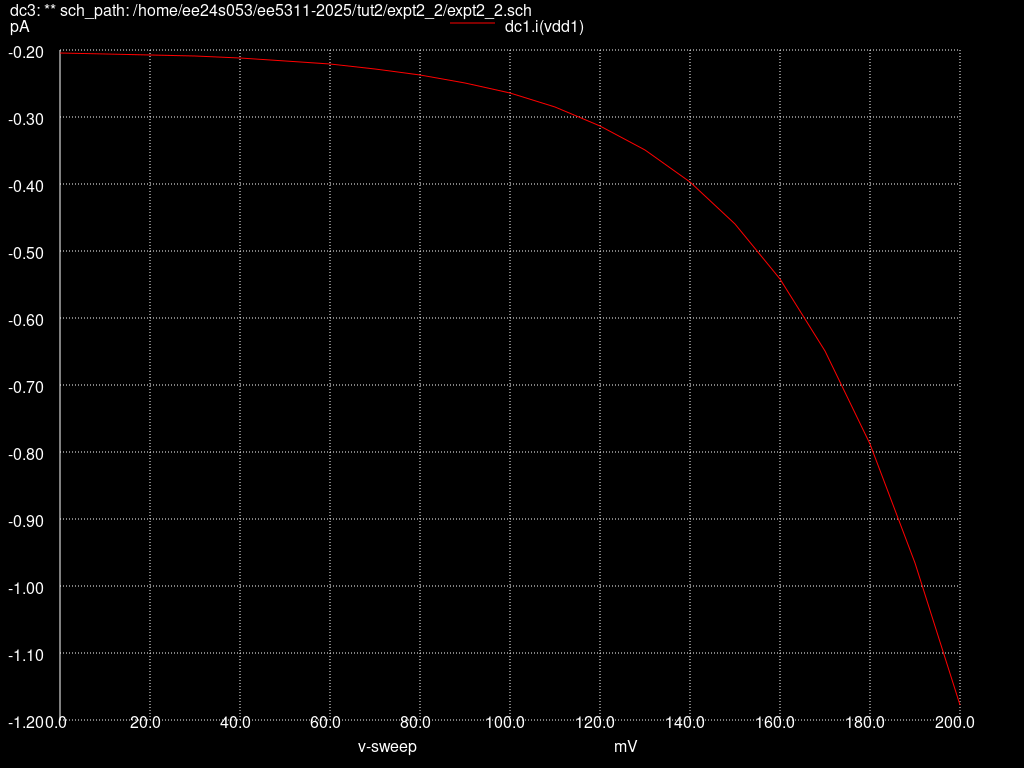
\includegraphics[scale=0.3]{tut2/reports/media/expt2_2_ids_0_2.png}
\end{center}

\begin{center}
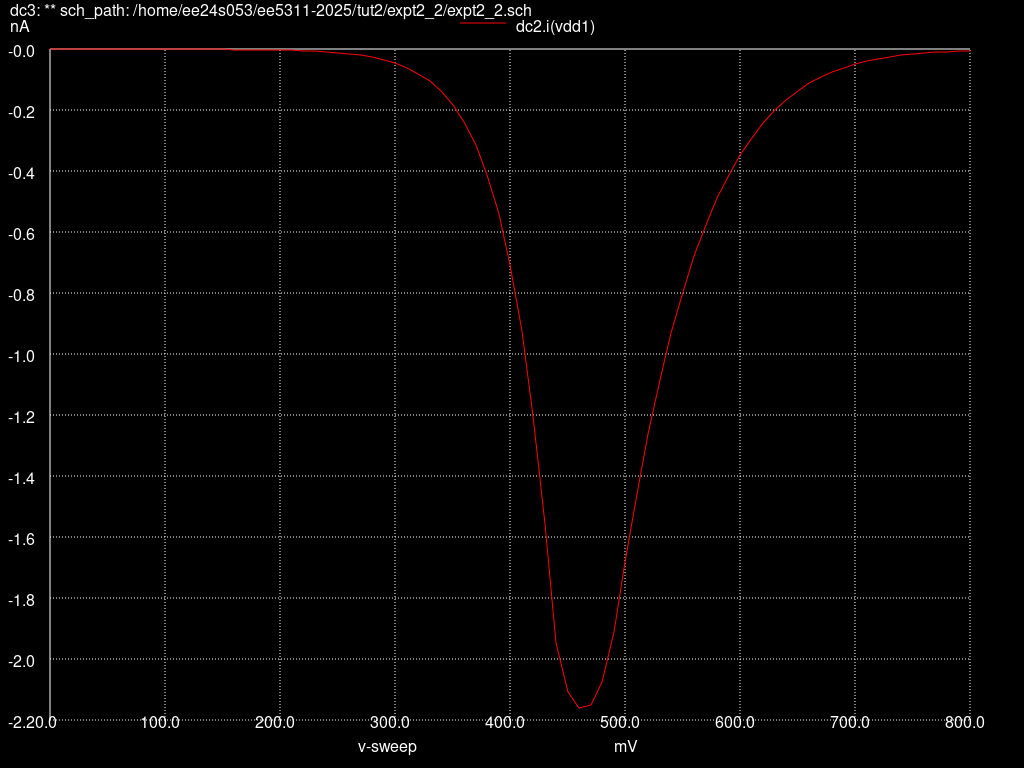
\includegraphics[scale=0.3]{tut2/reports/media/expt2_2_ids_0_8.png}
\end{center}

\begin{center}
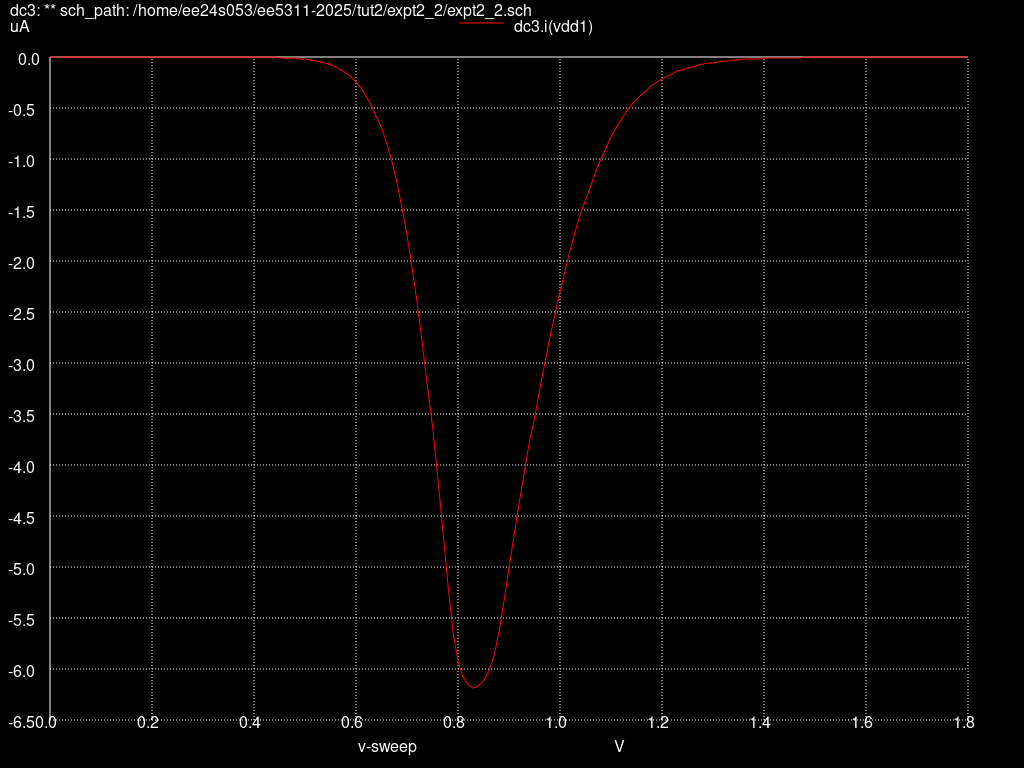
\includegraphics[scale=0.3]{tut2/reports/media/expt2_2_ids_1_8.png}
\end{center}

We make the following observations:

\end{document}
